\documentclass[11pt]{article}
\usepackage[margin=0.9in]{geometry}
\usepackage[T1]{fontenc}
\usepackage{lmodern}
\usepackage{graphicx}
\usepackage{booktabs}
\usepackage{float}
\usepackage{xcolor}
\usepackage{array}
\usepackage{tabularx}
\usepackage{url}
\usepackage[hidelinks]{hyperref}

\setlength{\parindent}{0pt}
\setlength{\parskip}{5pt}
\newcommand{\figwidth}{0.98\linewidth}

\title{\vspace{-1.4cm}EE291F Homework 1\\[2pt]
Cadence Genus Synthesis Flow for MohoTop (RISC-V)}
\author{Jichen Zhou\\Student ID: [2603000020]}
\date{November 17, 2026}

\begin{document}
\maketitle

\section{Objective}

Complete the five-stage Cadence Genus synthesis flow for the \texttt{MohoTop}
RISC-V processor and submit the synthesized netlist, the exported SDC, and the
\texttt{report\_summary} reports.

\section{Environment and Inputs}

\begin{table}[H]
\centering
\small
\begin{tabular}{@{}ll@{}}
\toprule
Item & Value \\
\midrule
Top module & \texttt{MohoTop} (RV32I, five-stage pipeline) \\
Clock & \texttt{io\_pins\_clk}, 6.667 ns (150 MHz) \\
Reset & \texttt{io\_pins\_rst} \\
Memories & 2 $\times$ \path{mem_hl55_2048x32_sp_m1} \\
Technology & HL055P\_7M6X1T4\_RDL, RVT + LVT standard cells \\
Process library & \path{/mnt/nfs_share/EE291F/3003/tech.prj} \\
Synthesis tool & Cadence Genus 25.10-p002\_1 \\
\bottomrule
\end{tabular}
\end{table}

The RTL and SDC were copied unchanged from the course project
(\path{/mnt/nfs_share/EE291F/3003/FlowPrjRISCV}). The flow is Make-driven: the
\texttt{tech} symlink is created by \texttt{make init}, and each stage is a Tcl
script under \texttt{script/genus/}.

\section{Flow and Stage Results}

The five stages were run in order. Clock uncertainty was tightened during
optimization (1.25, 1.00, and 0.75 ns setup for generic, map, and opt) and then
restored to the original 0.50 ns in the final stage, as required by the
assignment. All stages finished with \texttt{Normal exit}. The figures below are
terminal transcripts rendered from the recorded run logs; each shows the command
executed, the main tool messages, and the success line.

\begin{table}[H]
\centering
\small
\begin{tabular}{@{}lll@{}}
\toprule
Stage & Command & Main action \\
\midrule
01\_elaborate & \texttt{make genus-elaborate} & Read MMMC/LEF/RTL, elaborate, apply constraints \\
02\_generic & \texttt{make genus-generic} & \texttt{syn\_generic} \\
03\_map & \texttt{make genus-map} & \texttt{syn\_map} \\
04\_opt & \texttt{make genus-opt} & \texttt{syn\_opt} \\
05\_final & \texttt{make genus-final} & Export netlist/SDC, collect reports \\
\bottomrule
\end{tabular}
\end{table}

\subsection{Stage 01: Elaborate}

The MMMC, LEF, and RTL were read, and the design was elaborated. The clock and
reset networks were protected with \texttt{set\_dont\_touch\_network}, and the
dont-use cell patterns were applied. \texttt{check\_design -unresolved} reports
no unresolved references and no empty modules. Generated files:
\texttt{MohoTop.db}, \texttt{netlist.v}, and \texttt{check\_design.rpt}.

\begin{figure}[H]
\centering
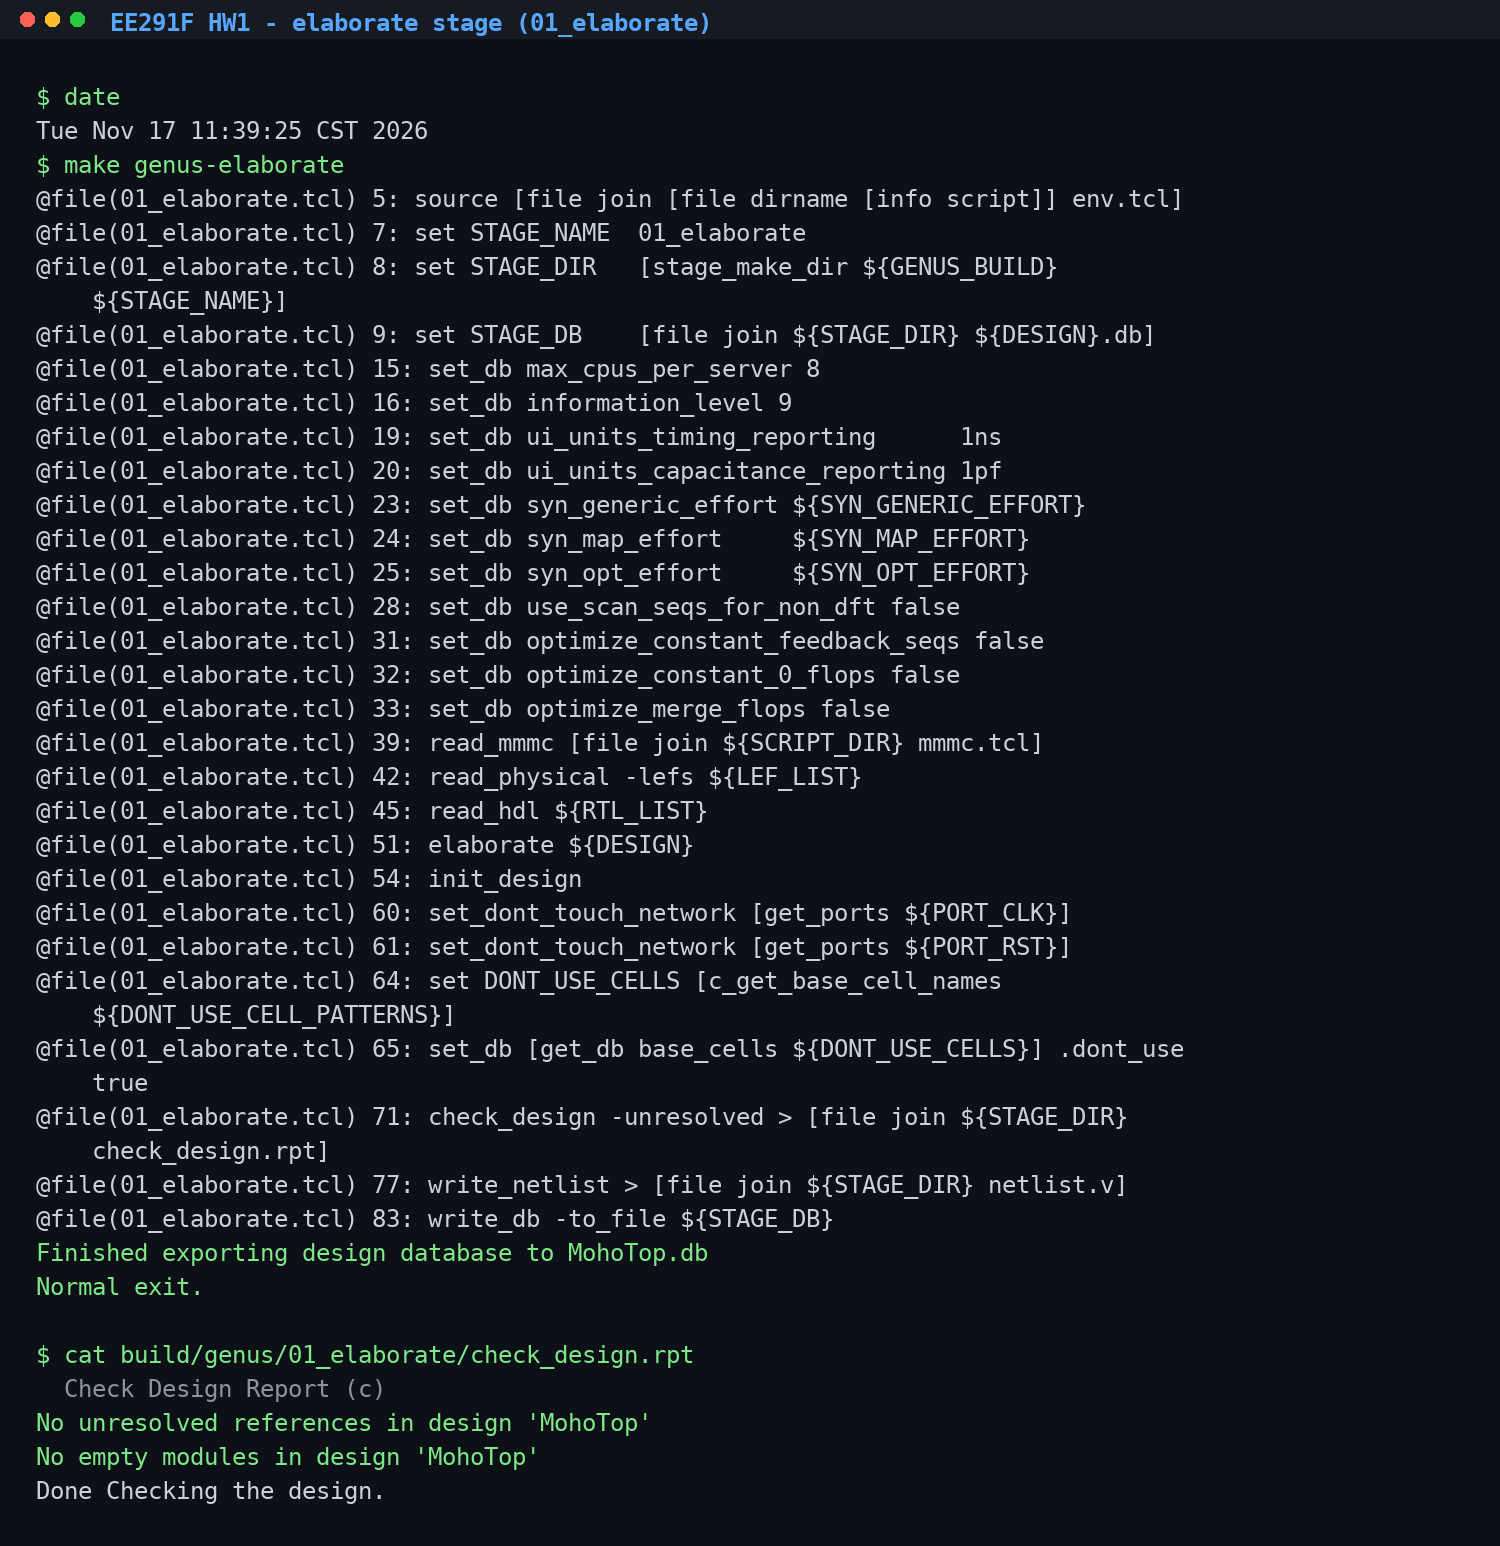
\includegraphics[width=\figwidth]{figures/stage_01_elaborate.png}
\caption{Elaborate stage: command, elaboration flow, and clean check\_design report.}
\end{figure}

\subsection{Stage 02: Generic}

The stage restored the elaborate database, applied 1.25 ns setup / 0.05 ns hold
uncertainty, and ran \texttt{syn\_generic}. The design had 17{,}288 leaf
instances after this stage. Generated files: \texttt{MohoTop.db},
\texttt{netlist.v}, and \texttt{syn\_generic\_*.rpt}.

\begin{figure}[H]
\centering
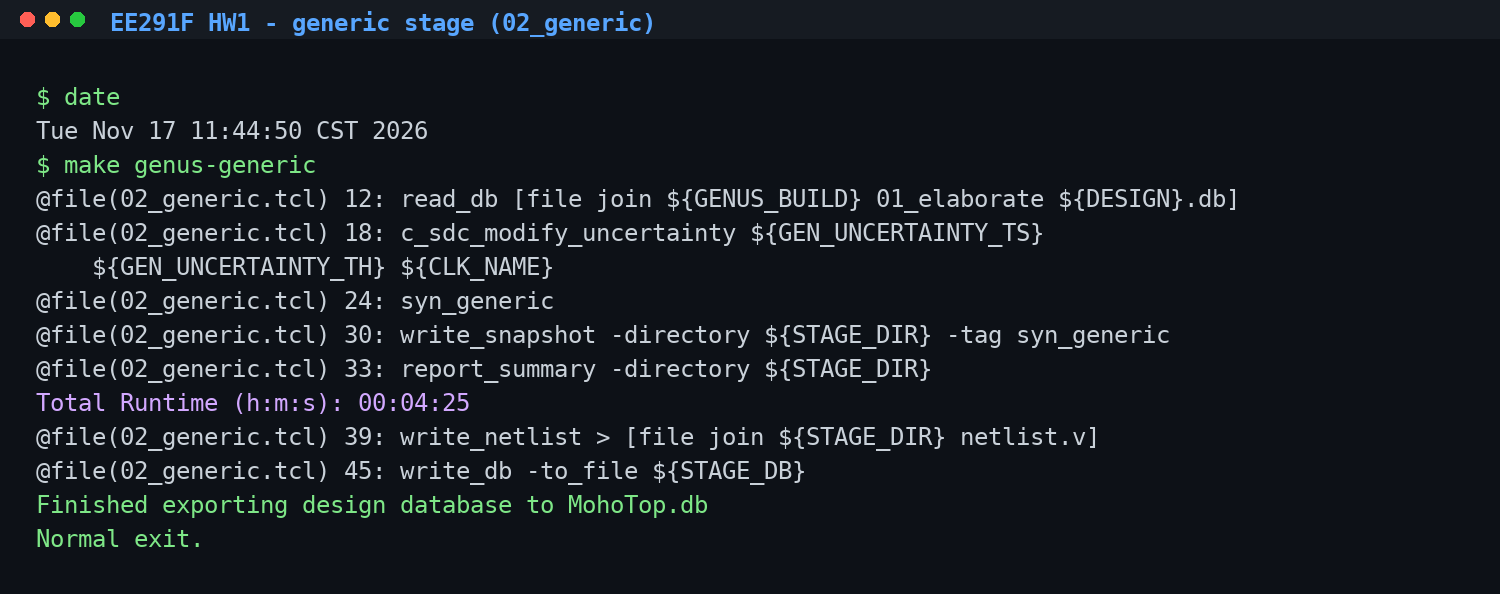
\includegraphics[width=\figwidth]{figures/stage_02_generic.png}
\caption{Generic stage: \texttt{syn\_generic} completed successfully.}
\end{figure}

\subsection{Stage 03: Map}

The generic database was restored, uncertainty was tightened to 1.00 ns, and
\texttt{syn\_map} mapped the design to HL55 standard cells. The worst
\texttt{view\_ss\_ccw} slack was +0.001 ns after mapping. Generated files:
\texttt{MohoTop.db}, \texttt{netlist.v}, and \texttt{syn\_map\_*.rpt}.

\begin{figure}[H]
\centering
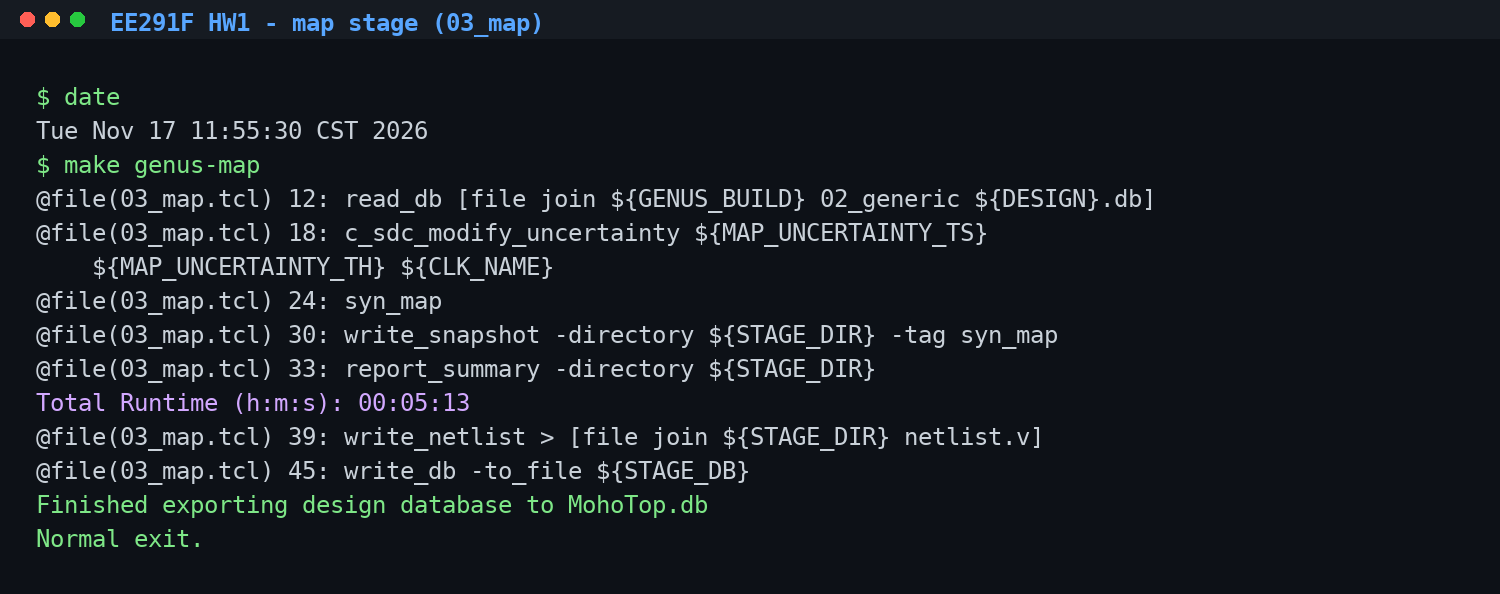
\includegraphics[width=\figwidth]{figures/stage_03_map.png}
\caption{Map stage: \texttt{syn\_map} completed successfully.}
\end{figure}

\subsection{Stage 04: Opt}

The mapped database was restored, uncertainty was set to 0.75 ns, and
\texttt{syn\_opt} optimized the mapped netlist. The design had 10{,}290 leaf
instances and no failing paths. Generated files: \texttt{MohoTop.db},
\texttt{netlist.v}, and \texttt{syn\_opt\_*.rpt}.

\begin{figure}[H]
\centering
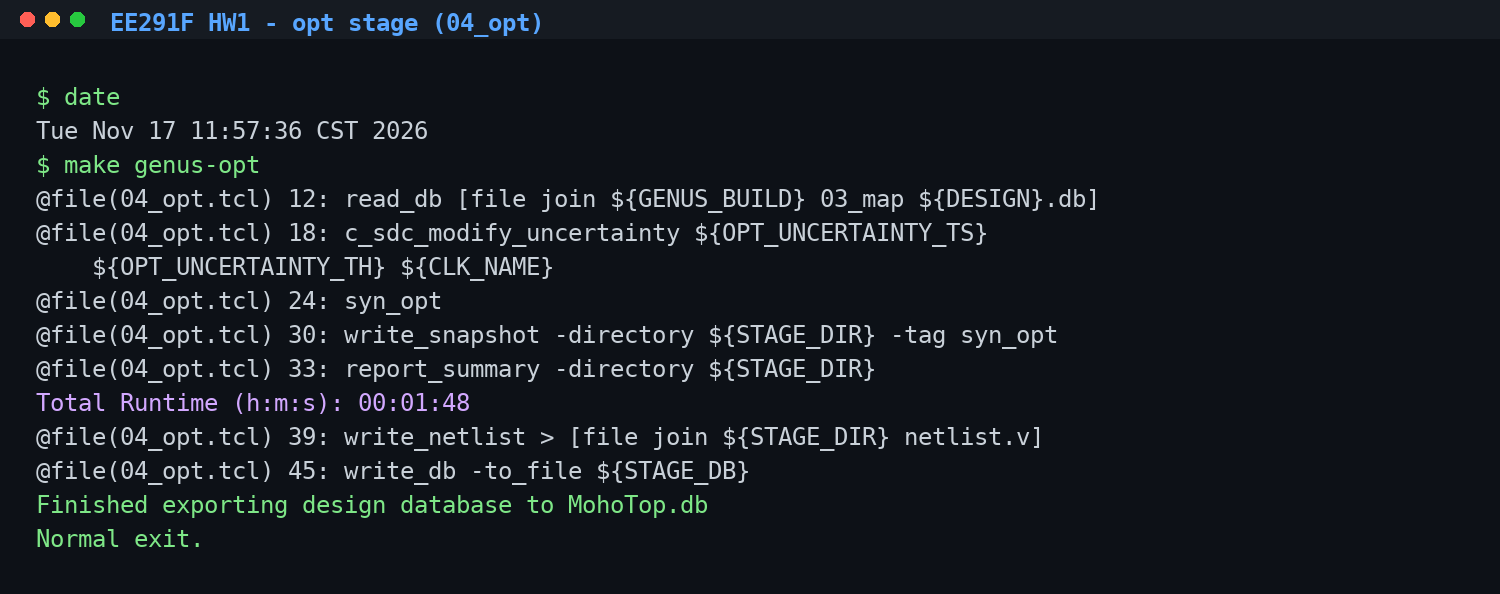
\includegraphics[width=\figwidth]{figures/stage_04_opt.png}
\caption{Opt stage: \texttt{syn\_opt} completed successfully.}
\end{figure}

\subsection{Stage 05: Final}

The optimized database was restored, uncertainty was returned to the original
0.50 ns, and the final snapshot and report summary were written. The netlist
\path{MohoTop_syn.v} and constraints \path{MohoTop_syn_func_main.sdc} were
exported and copied to \path{netlist/}; all \texttt{*.rpt} files were copied to
\path{reports/}. The final design has no failing paths in either view.

\begin{figure}[H]
\centering
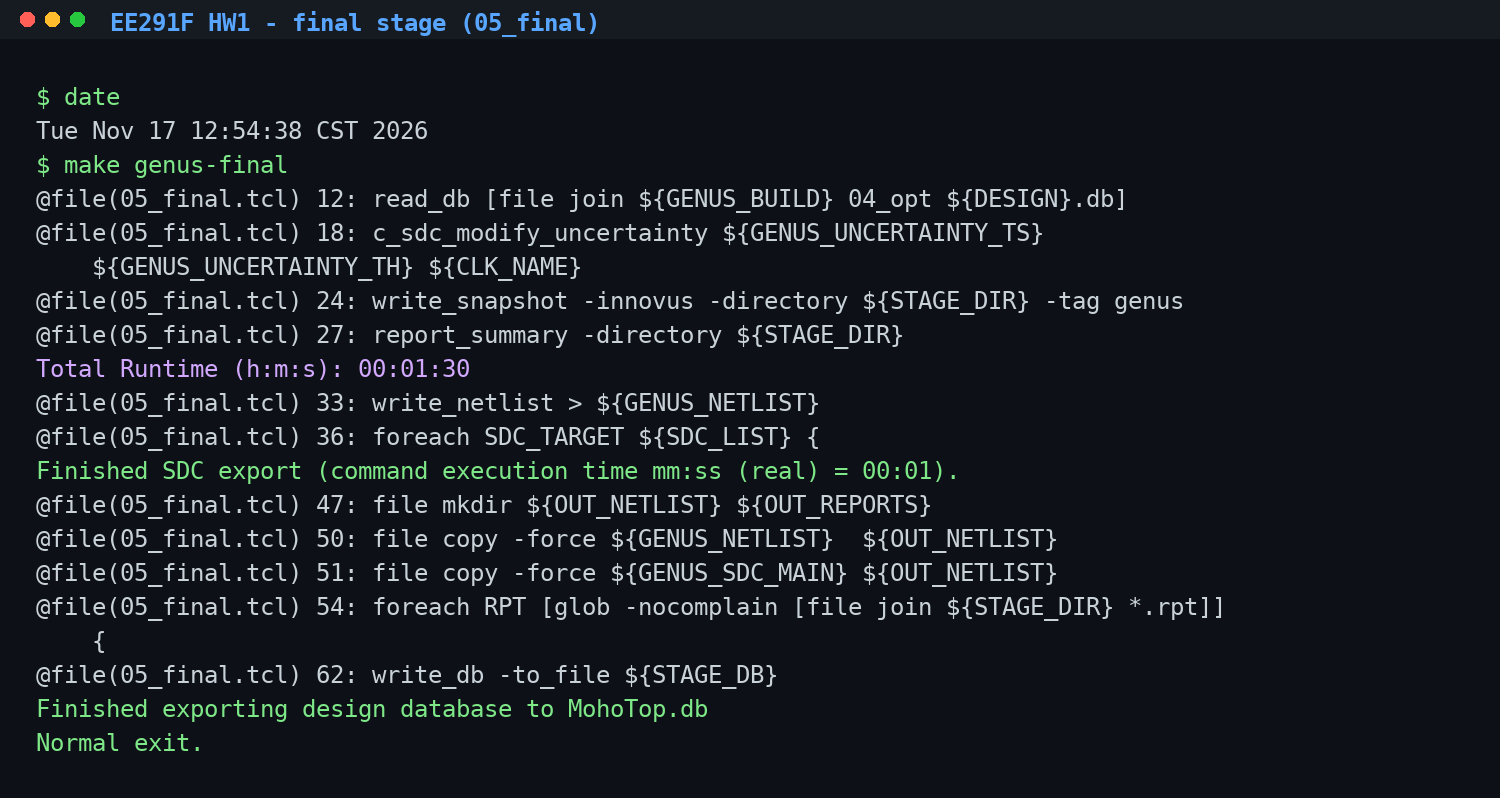
\includegraphics[width=\figwidth]{figures/stage_05_final.png}
\caption{Final stage: netlist/SDC export and deliverable collection.}
\end{figure}

\section{Final Deliverables}

The final file listing is shown below. The report PDF, netlist, SDC, and reports
are non-empty and come from the same complete run.

\begin{figure}[H]
\centering
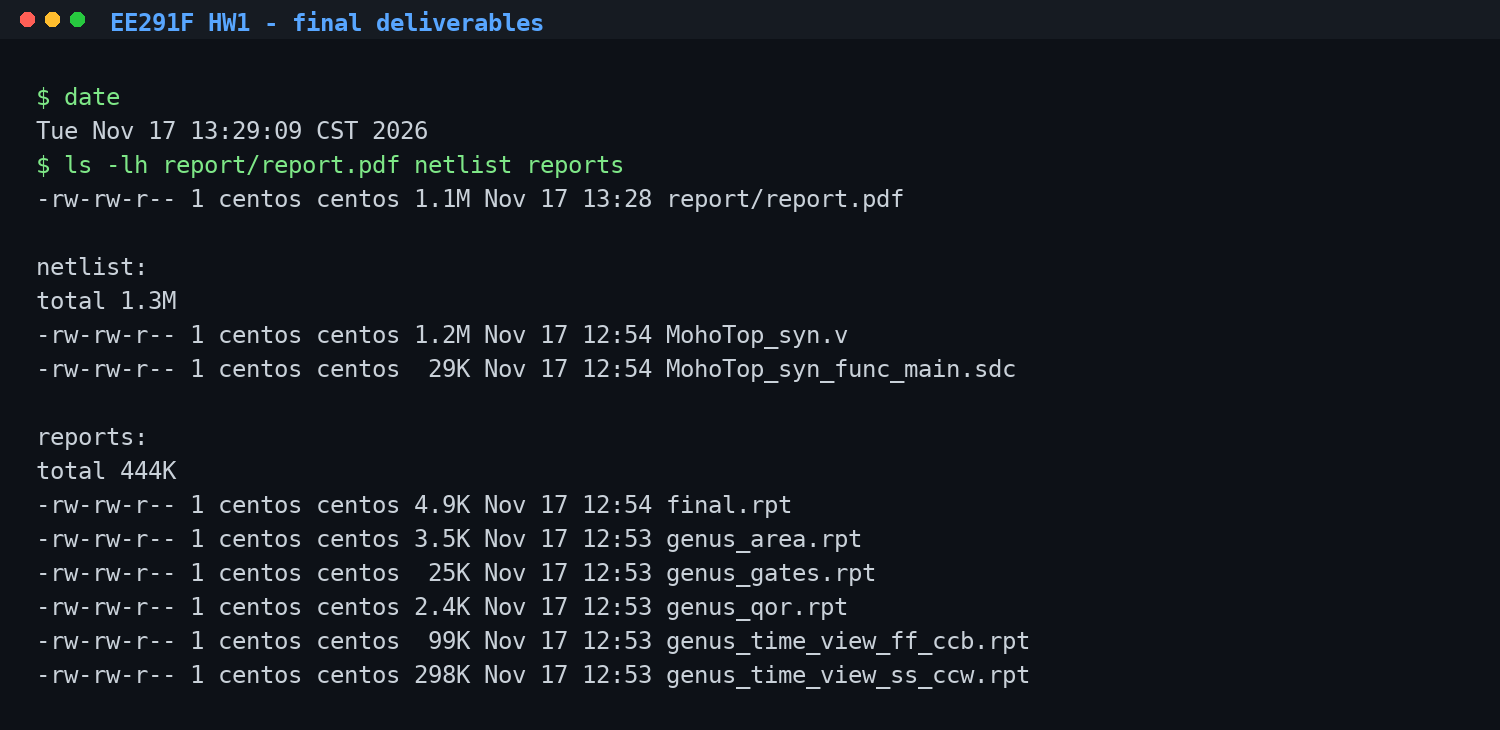
\includegraphics[width=\figwidth]{figures/deliverables.png}
\caption{Final \texttt{ls -lh report/report.pdf netlist reports} output.}
\end{figure}

\begin{table}[H]
\centering
\small
\begin{tabular}{@{}llr@{}}
\toprule
Directory & File & Size \\
\midrule
\texttt{report/} & \texttt{report.pdf} & 1.1 MB \\
\texttt{netlist/} & \texttt{MohoTop\_syn.v} & 1.2 MB \\
\texttt{netlist/} & \texttt{MohoTop\_syn\_func\_main.sdc} & 29 KB \\
\texttt{reports/} & \texttt{genus\_qor.rpt} & 2.4 KB \\
\texttt{reports/} & \texttt{genus\_area.rpt} & 3.5 KB \\
\texttt{reports/} & \texttt{genus\_gates.rpt} & 25 KB \\
\texttt{reports/} & \texttt{genus\_time\_view\_ss\_ccw.rpt} & 298 KB \\
\texttt{reports/} & \texttt{genus\_time\_view\_ff\_ccb.rpt} & 99 KB \\
\texttt{reports/} & \texttt{final.rpt} & 4.9 KB \\
\bottomrule
\end{tabular}
\end{table}

\section{Timing and Area Results}

Timing is met in both analysis views with no violating paths (Table~\ref{tab:finaltiming}).
The slack progression across the flow is summarized in Table~\ref{tab:progress}.

\begin{table}[H]
\centering
\small
\caption{Final timing at the original 0.50 ns uncertainty.}
\label{tab:finaltiming}
\begin{tabular}{@{}lrrr@{}}
\toprule
View & Setup slack (ns) & TNS (ns) & Failing paths \\
\midrule
\texttt{view\_ss\_ccw} & +0.250 & 0.000 & 0 \\
\texttt{view\_ff\_ccb} & +1.887 & 0.000 & 0 \\
\bottomrule
\end{tabular}
\end{table}

\begin{table}[H]
\centering
\small
\caption{Slack and area progression across the flow.}
\label{tab:progress}
\begin{tabular}{@{}lrrr@{}}
\toprule
Stage & \texttt{ss\_ccw} slack (ns) & \texttt{ff\_ccb} slack (ns) & Cell area \\
\midrule
\texttt{syn\_generic} & 0.036 & 1.249 & 108{,}090 \\
\texttt{syn\_map} & 0.001 & 1.387 & 152{,}781 \\
\texttt{syn\_opt} & 0.000 & 1.637 & 151{,}034 \\
\texttt{genus} (final) & 0.250 & 1.887 & 151{,}034 \\
\bottomrule
\end{tabular}
\end{table}

Final area and instance counts from \texttt{genus\_qor.rpt}: cell area
151{,}033.906, net area 18{,}601.297, total area 169{,}635.203; 10{,}290 leaf
instances (2{,}415 sequential, 7{,}875 combinational, 28 hierarchical).

\begin{verbatim}
view_ss_ccw  main_clk  0.250  0.000  0
view_ff_ccb  main_clk  1.887  0.000  0
Cell Area                          151033.906
Leaf Instance Count                   10290
Normal exit.
\end{verbatim}

\section{Version Control Workflow}

Git was used to manage the flow: the scaffold, Makefile and Genus targets,
configuration fixes, the five stage scripts, and the report were committed as
the work progressed. The complete project, including the RTL, Tcl scripts,
synthesized netlist and reports, and this report, is publicly available on
GitHub:

\begin{center}
\url{https://github.com/pineklll/HW1-Cadence-Genus-Synthesis-Flow-for-MohoTop}
\end{center}

The recorded commits are:

{\footnotesize
\begin{verbatim}
cd5b22b  2026-11-12  Initial commit
9225c82  2026-11-12  Scaffold MohoTop Genus synthesis flow
421d80b  2026-11-17  Update Makefile for MohoTop Genus flow
d224fe0  2026-11-17  Add tool-genus.mk
2723081  2026-11-17  Include tool-genus.mk in Makefile
181d25a  2026-11-17  Fix Makefile line 38 syntax error
7001be5  2026-11-17  Complete Tcl scripts; update tech/design config
b3e279c  2026-11-17  Finish tech.tcl and 01_elaborate.tcl
de59744  2026-11-17  Finish remaining stages and report
11e138c  2026-11-17  Add student ID, LaTeX ignores, clean root
fbee29c  2026-11-17  Include report PDF in deliverables screenshot
\end{verbatim}
}

The commit history above records the development of the flow; the final
deliverables are tracked in the same repository.

\section{Conclusion}

All five required stages completed successfully, and timing is met in both
corners. The final netlist, exported SDC, and \texttt{report\_summary} reports
are in the submission layout under \texttt{netlist/} and \texttt{reports/}. The
flow is reproducible with \texttt{make init} followed by the five stage targets.

\end{document}